\chapter{Redes ad-hoc}
\section{O que é Ad Hoc?}
\paragraph{} Ad Hoc é uma expressão oriunda do latim que significa "para isso", no sentido de finalidade, propósito \citep{Latim2014}. Apesar desse nome, no mundo das telecomunicações e redes de computadores, redes Ad Hoc ou MANET (\textit{Mobile Ad hoc NETwork}) esses, são tipos de redes que não possuem um ponto de acesso. 

\paragraph{} Para que essa definição seja viável, a rede deverá ser sem fio e com terminais capazes de estabelecer e gerenciar as comunicações dentro da rede. Como poderá ser visto no capítulo 3, os dispositivos integrantes da rede Ad Hoc desempenham funções de roteamento e de expansão da rede ao estabelecer conexão com novos terminais. A figura \ref{fig:figura1} ilustra uma rede Ad Hoc simples.

\begin{figure}[!ht]
	\centering
	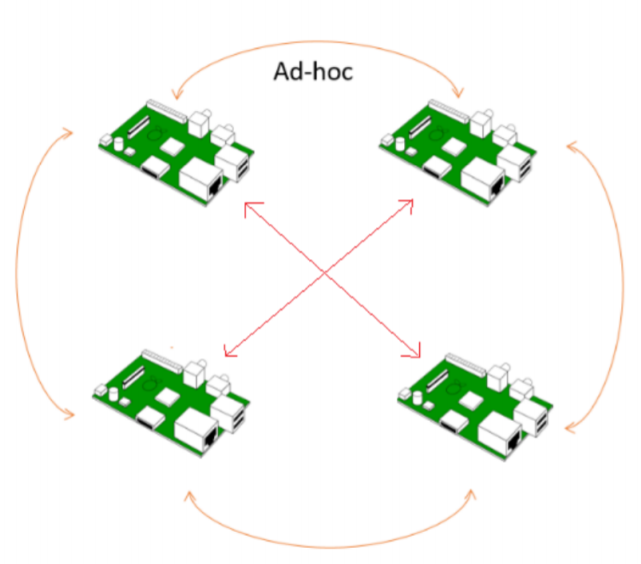
\includegraphics[width=0.4\textwidth]{Figuras/ad-hoc.PNG}   
	\caption{Exemplo de rede Ad Hoc.}
	\label{fig:figura1}
\end{figure}

\paragraph{} Atualmente a concepção de rede Ad Hoc é bastante utilizada, e se faz presente em diversas tecnologias de grande importância no dia a dia das pessoas. Um grande exemplo de rede Ad Hoc é o \textit{Bluetooth}, onde são usados, por exemplo, para comunicação de PCs com impressoras, mouses e teclados sem fio. 

\section{Histórico}
\paragraph{} As primeiras aparições de redes Ad Hoc foram datadas de 1972 em um projeto chamado \textit{Packet Radio Network} (PRNET) pela Agência de Investigação de Projetos Avançados de Defesa (DARPA), dos Estados Unidos.

\paragraph{} Em 1983 a DARPA, expandindo o PRNET, lançou o programa SURAN (\textit{Survivable Adaptive Network}), que foi de grande importância no suporte de grandes redes e no desenvolvimento de protocolos de rede adaptáveis às variações no meio.

\paragraph{} Um terceiro grande projeto sobre redes Ad Hoc foi o GloMo (\textit{Global Mobile Information Systems}), que teve início em 1994. Mais uma vez foi feito pela DARPA, esse projeto teve como grande diferencial o uso do padrão IEEE 802.11, o Wi-fi. Apesar da DARPA liderar essa inovação, o conceito de redes Ad Hoc já havia se expandido para o meio civil nessa época.

\section{Das Vantagens e Desvantagens}
\paragraph{} Vantagens:

\begin{itemize}
   \item Não precisa de uma estrutura fixa:  Otimizando o tempo e o custo de montagem, além de aumentar a mobilidade.
   \item Não apresenta terminais críticos:  A rede não é afetada se algum dispositivo falhar.
   \item Escalabilidade:  Novos terminais podem ser facilmente adicionados na rede.
   \item Conectividade: Dois nós quaisquer, podem se comunicar diretamente, se um estiver ao alcance do outro. 
   
\end{itemize}
 
\paragraph{} Desvantagens:
 
\begin{itemize}
   \item Menor alcance em relação a outros tipos de rede.
   \item Roteamento: A mobilidade dos nós e a topologia contribuem para aumentar o grau de complexidade do algoritmo de roteamento da rede.
   \item Por ser uma rede sem fio, a rede Ad Hoc também tem taxas de erros mais elevadas e menor banda passante do que as redes cabeadas.
\end{itemize}

\section{Redes Mesh}
\paragraph{} Entre as topologias aplicadas em redes MANET, a mais usada é a rede \textit{mesh}, uma rede em que os nós se conectam diretamente, dinamicamente e de maneira não hierárquica. Essa rede, pode ser representada pela seguinte figura:

\begin{figure}[!ht]
	\centering
	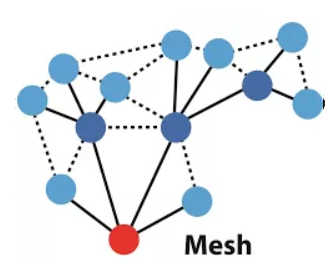
\includegraphics[width=0.4\textwidth]{Figuras/mesh.PNG}   
	\caption{Exemplo de rede \textit{mesh}. \citep{Mesh}}
	\label{fig:figura2}
\end{figure}

\paragraph{} Uma rede \textit{mesh} é caracterizada de duas formas, parcial e total. Na parcial nem todos os nós estão interconectados, já na forma total, ela apresenta todas as conexões possíveis. 

\paragraph{} Como essa rede dispõe de diversas conexões, para transmitir uma mensagem é preciso de técnicas de roteamento e algoritmos de auto-recuperação dos pacotes, em função dos diversos caminhos possíveis.